\documentclass[11pt,a4paper]{article}
%\usepackage{fontspec, xunicode, xltxtra}  
%\setmainfont{Hiragino Sans GB}  
\usepackage{xeCJK}
%\setCJKmainfont[BoldFont=STZhongsong, ItalicFont=STKaiti]{STSong}
%\setCJKsansfont[BoldFont=STHeiti]{STXihei}
%\setCJKmonofont{STFangsong}

%使用Xelatex编译

% 设置页面
%==================================================
\linespread{2} %行距
% \usepackage[top=1in,bottom=1in,left=1.25in,right=1.25in]{geometry}
% \headsep=2cm
% \textwidth=16cm \textheight=24.2cm
%==================================================

% 其它需要使用的宏包
%==================================================
\usepackage[colorlinks,linkcolor=blue,anchorcolor=red,citecolor=green,urlcolor=blue]{hyperref} 
\usepackage{tabularx}
\usepackage{authblk}         % 作者信息
\usepackage{algorithm}     % 算法排版
\usepackage{amsmath}     % 数学符号与公式
\usepackage{amsfonts}     % 数学符号与字体
\usepackage{mathrsfs}      % 花体
\usepackage{amssymb}
\usepackage[framemethod=TikZ]{mdframed}

\usepackage{graphicx} 
\usepackage{graphics}
\usepackage{color}
\usepackage{xcolor}
\usepackage{tcolorbox}
\usepackage{lipsum}
\usepackage{empheq}

\usepackage{fancyhdr}       % 设置页眉页脚
\usepackage{fancyvrb}       % 抄录环境
\usepackage{float}              % 管理浮动体
\usepackage{geometry}     % 定制页面格式
\usepackage{hyperref}       % 为PDF文档创建超链接
\usepackage{lineno}          % 生成行号
\usepackage{listings}        % 插入程序源代码
\usepackage{multicol}       % 多栏排版
%\usepackage{natbib}         % 管理文献引用
\usepackage{rotating}       % 旋转文字,图形,表格
\usepackage{subfigure}    % 排版子图形
\usepackage{titlesec}       % 改变章节标题格式
\usepackage{moresize}   % 更多字体大小
\usepackage{anysize}
\usepackage{indentfirst}  % 首段缩进
\usepackage{booktabs}   % 使用\multicolumn
\usepackage{multirow}    % 使用\multirow

\usepackage{wrapfig}
\usepackage{titlesec}     % 改变标题样式
\usepackage{enumitem}
\usepackage{aas_macros}
\usepackage{bigints}

\renewcommand{\vec}[1]{\boldsymbol{#1}}
\newcommand{\me}{\mathrm{e}}
\newcommand{\mi}{\mathrm{i}}
\newcommand{\dif}{\mathrm{d}}
\newcommand{\tabincell}[2]{\begin{tabular}{@{}#1@{}}#2\end{tabular}}

\def\kpc{{\rm kpc}}
\def\km{{\rm km}}
\def\cm{{\rm cm}}
\def\TeV{{\rm TeV}}
\def\GeV{{\rm GeV}}
\def\MeV{{\rm MeV}}
\def\GV{{\rm GV}}
\def\MV{{\rm MV}}
\def\yr{{\rm yr}}
\def\s{{\rm s}}
\def\ns{{\rm ns}}
\def\GHz{{\rm GHz}}
\def\muGs{{\rm \mu Gs}}
\def\arcsec{{\rm arcsec}}
\def\K{{\rm K}}
\def\microK{\mu{\rm K}}
\def\sr{{\rm sr}}
\newcolumntype{p}{D{,}{\pm}{-1}}

\renewcommand{\figurename}{Fig.}
\renewcommand{\tablename}{Tab.}

\renewcommand{\arraystretch}{1.5}

\setlength{\parindent}{0pt}  %取消每段开头的空格

\newcounter{theo}[section]\setcounter{theo}{0}
\renewcommand{\thetheo}{\arabic{section}.\arabic{theo}}
\newenvironment{theo}[2][]{%
\refstepcounter{theo}%
\ifstrempty{#1}%
{\mdfsetup{%
frametitle={%
\tikz[baseline=(current bounding box.east),outer sep=0pt]
\node[anchor=east,rectangle,fill=blue!20]
{\strut Theorem~\thetheo};}}
}%
{\mdfsetup{%
frametitle={%
\tikz[baseline=(current bounding box.east),outer sep=0pt]
\node[anchor=east,rectangle,fill=blue!20]
{\strut Theorem~\thetheo:~#1};}}%
}%
\mdfsetup{innertopmargin=10pt,linecolor=blue!20,%
linewidth=2pt,topline=true,%
frametitleaboveskip=\dimexpr-\ht\strutbox\relax
}
\begin{mdframed}[]\relax%
\label{#2}}{\end{mdframed}}

\newcommand*\widefbox[1]{\fbox{\hspace{2em}#1\hspace{2em}}}


\title{微振动}
\author{}
\date{\today}
\begin{document}

\maketitle

\section{一维自由振动}
\cite{2007理论物理学教程} 在稳定平衡位置附近的运动称为微振动。稳定平衡位置是指势能$U(q)$取极小值的位置,偏离该位置会导致产生力$-\dfrac{\dif U}{\dif q}$,它力图使系统返回平衡位置。用$q_0$表示广义坐标$q$在平衡位置的值。在偏离平衡位置很小的情况下,在$U(q)-U(q_0)$按$q-q_0$的幂次展开,
\begin{equation*}
U(q) - U(q_0) \approx \dfrac{k}{2} (q-q_0)^2 ~,
\end{equation*}
$k$是二阶导数$U^{\prime \prime}(q)$在$q =q_0$处的值,是正数。





\section{强迫振动}
\cite{2007理论物理学教程} 可变外力场作用下系统的振动,称为\textcolor{red}{强迫振动}。


强迫力是频率为$\gamma$的简单时间周期函数,即
\begin{equation}
F(t) = f \cos(\gamma t +\beta) ~.
\end{equation}

\begin{equation}
x = a\cos (\omega t +\alpha) +\dfrac{f}{m(\omega^2 -\gamma^2)} \cos(\gamma t +\beta) ~.
\end{equation}
任意积分常数$a$和$\alpha$由初始条件确定。在周期性强迫力作用下,系统的运动是两个振动的合成,两个振动的频率分别为系统的固有频率$\omega$和强迫力的频率$\gamma$。以上不适用于共振情况,即强迫力的频率$\gamma$与固有频率$\omega$相等。
\begin{equation}
x = a\cos (\omega t +\alpha) +\dfrac{f}{m(\omega^2 -\gamma^2)} [ \cos(\gamma t +\beta) -\cos(\omega t +\beta)] ~.
\end{equation}
当$\gamma \rightarrow \omega$,可得
\begin{equation}
x = a\cos (\omega t +\alpha) +\dfrac{f}{2m \omega} t \sin(\omega t +\beta) ~.
\end{equation}
在共振情况下,振动的振幅随时间线性增长。





\section{多自由度系统振动}
\cite{2007理论物理学教程} 






\section{分子振动}
\cite{2007理论物理学教程} 













\section{阻尼振动}
\cite{2007理论物理学教程} 



若速度足够小,可以将摩擦力按速度的幂次展开。作用在广义坐标为$x$的一维微振动系统的广义摩擦力$f_{\rm fr} $写成
\begin{equation}
f_{\rm fr} = -\alpha \dot{x} ~,
\end{equation}
$\alpha$为正的系数,

\begin{align}
& m \ddot{x} = -kx -\alpha \dot{x} ~, \\
& \dfrac{k}{m} = \omega_0^2 ~, \dfrac{\alpha}{m} = 2 \lambda ~.
\end{align}
$\omega_0$是没有摩擦力时系统自由振动的频率。$\lambda$称为\textcolor{red}{阻尼系数},或\textcolor{red}{阻尼衰减率}。$\lambda T$($T = 2\pi/\omega$是周期)称为\textcolor{red}{对数阻尼衰减率}。

\begin{equation}
\ddot{x} + 2\lambda \dot{x} +\omega_0^2 x = 0 ~.
\end{equation}
假设$x = e^{rt}$可得关于$r$的特征方程
\begin{equation*}
r^2 +2\lambda r + \omega_0^2 = 0 ~.
\end{equation*}
通解为
\begin{align*}
& x = c_1 e^{r_1 t} +c_2 e^{r_2 t} ~, \\
& r_{1, 2} = -\lambda \pm \sqrt{\lambda^2 -\omega_0^2} ~.
\end{align*}








\section{有摩擦的强迫振动}
\cite{2007理论物理学教程} 



















\section{参变振动}
\cite{2007理论物理学教程} 















\section{非简谐振动}
\cite{2007理论物理学教程} 









\section{非线性振动中的共振}
\cite{2007理论物理学教程} 







\section{快速振动场中的运动}
\cite{2007理论物理学教程} 









\section{pendulum}
\cite{morin2008introduction} \textbf{Pendulum with an oscillating support}. A pendulum consists of a mass $m$ and a massless stick of length $\ell$. The pendulum support oscillates horizontally with a position given by $x(t) = A \cos(\omega t)$ (see Fig. \ref{fig:oscillating_pen}). Calculate the angle of the pendulum as a function of time.



%===========================================================================================================================
\begin{figure*}
\centering
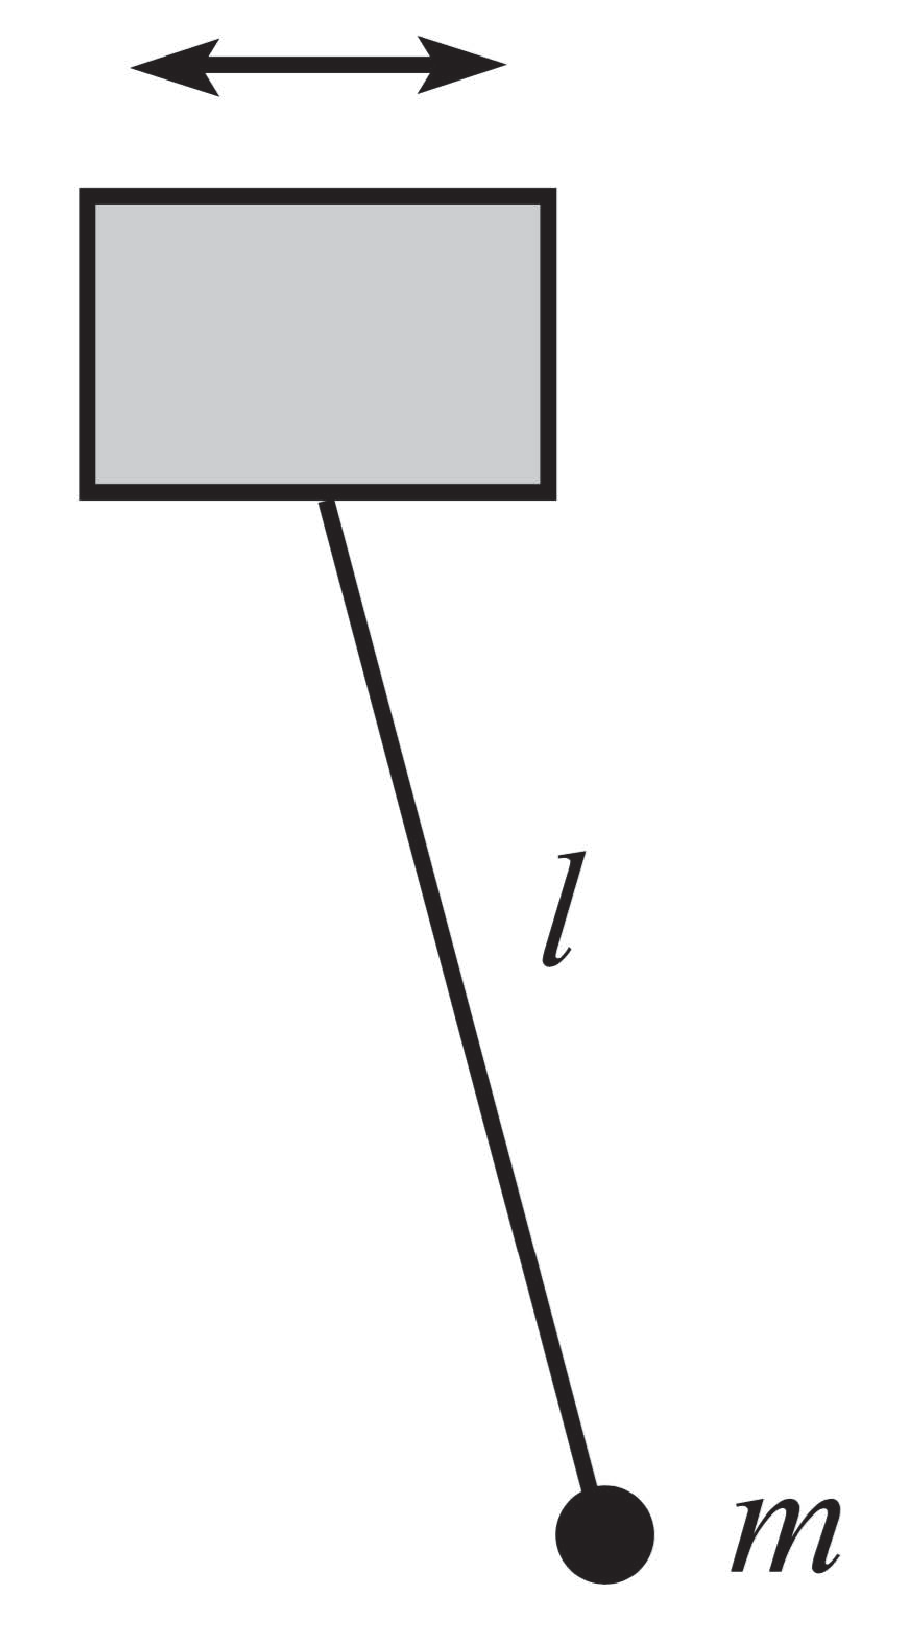
\includegraphics[height=4.cm, angle=0]{oscillating_pen.eps}
\caption{Pendulum with an oscillating support.
}
\label{fig:oscillating_pen}
\end{figure*}
%===========================================================================================================================

\cite{morin2008introduction} \textbf{Inverted pendulum}. A pendulum consists of a mass $m$ at the end of a massless stick of length $\ell$. The other end of the stick is made to oscillate vertically with a position given by $y(t) = A \cos(\omega t)$, where $A \ll \ell$. See Fig. \ref{fig:inverted_pen}. It turns out that if $\omega$ is large enough, and if the pendulum is initially nearly upside-down, then it will surprisingly not fall over as time goes by. Instead, it will (sort of) oscillate back and forth around the vertical position. Find the equation of motion for the angle of the pendulum (measured relative to its upside-down position). And explain why the pendulum doesn’t fall over, and find the frequency of the back and forth motion.

%===========================================================================================================================
\begin{figure*}
\centering
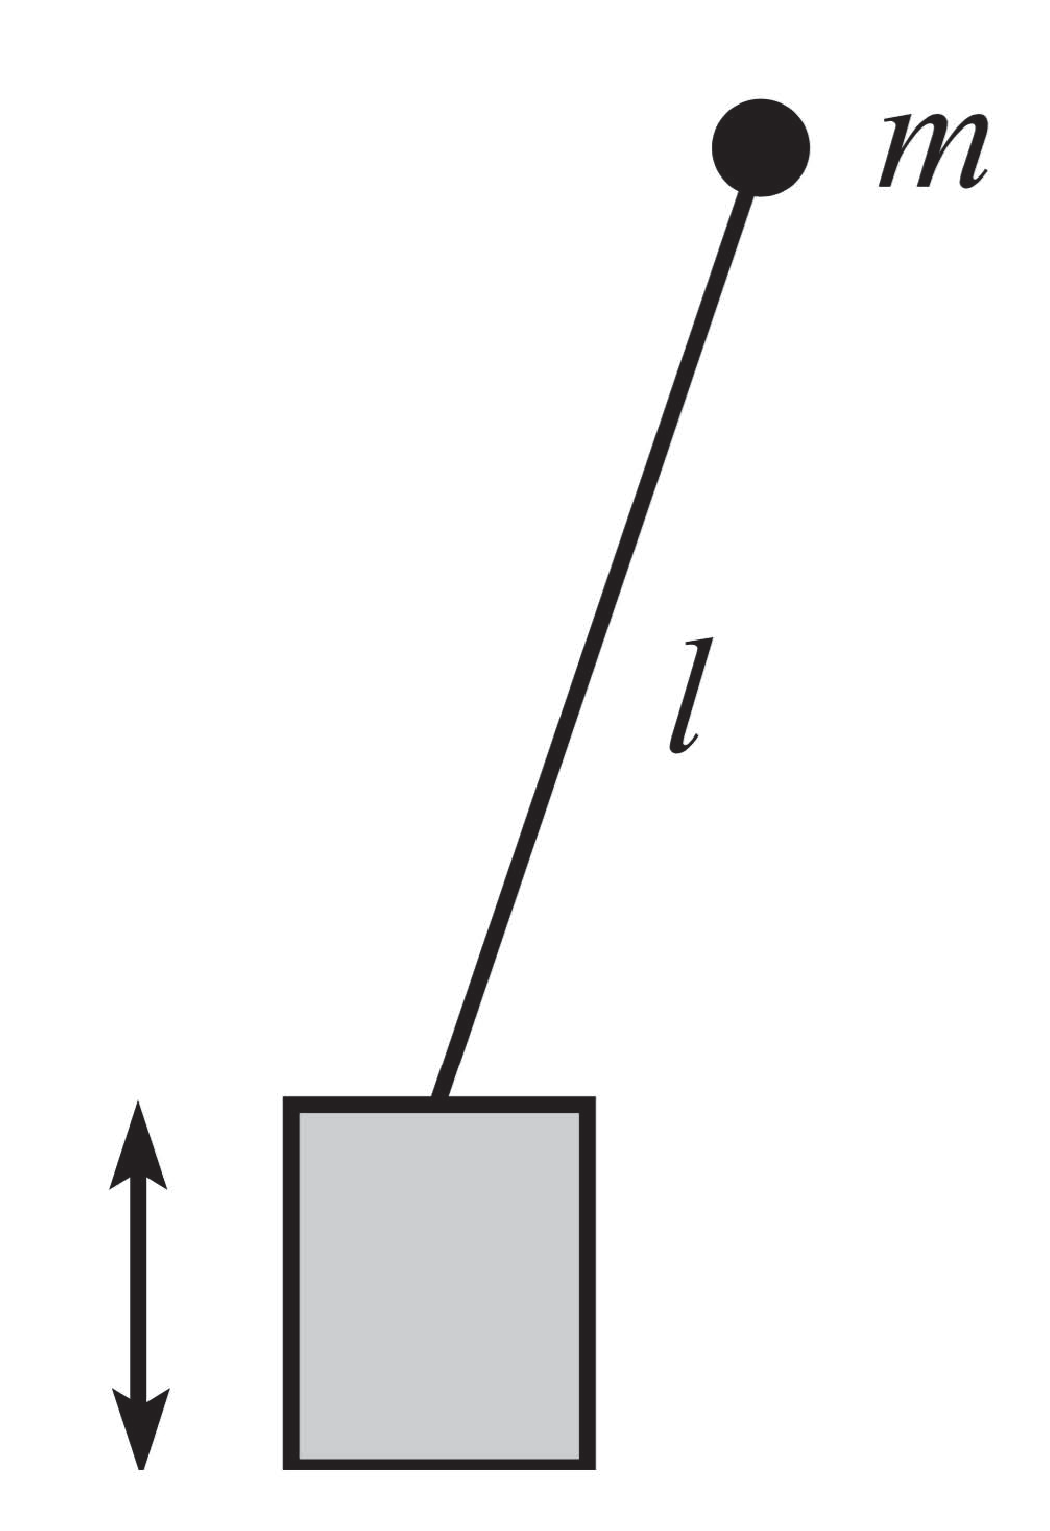
\includegraphics[height=4.cm, angle=0]{inverted_pen.eps}
\caption{Inverted pendulum.
}
\label{fig:inverted_pen}
\end{figure*}
%===========================================================================================================================

With $y(t) = A \cos(\omega t)$, the position of the mass m is given by 
\begin{equation}
(X, Y ) = (\ell \sin \theta, y + \ell \cos \theta) ~.
\end{equation}
Taking the derivatives of these coordinates, we see that the square of the speed is
\begin{equation}
V^2 = \dot{X}^2 + \dot{Y}^2 = \ell^2 \dot{\theta}^2 +\dot{y}^2 - 2 \ell \dot{y} \dot{\theta} \sin \theta ~.
\end{equation}
The Lagrangian is
\begin{equation}
L= \dfrac{1}{2} m( \ell^2 \dot{\theta}^2 + \dot{y}^2 - 2 \ell \dot{y} \dot{\theta} \sin \theta) -mg(y+\ell \cos \theta) ~. 
\end{equation}
The equation of motion for $\theta$ is
\begin{align}
\dfrac{\dif }{\dif t} \left(\dfrac{\partial L}{\partial \dot{\theta}} \right) &= \dfrac{\partial L}{\partial \theta} ~, \\
\ell \ddot{\theta} - \ddot{y} \sin \theta &= g \sin \theta ~.
\end{align}
Plugging in the explicit form of $y(t)$, we have
\begin{equation}
\ell \ddot{\theta} +\sin \theta \left( A\omega^2 \cos(\omega t) - g \right) = 0 ~.
\label{eq:inverted_1}
\end{equation}
In retrospect, this makes sense. Someone in the reference frame of the support, which has acceleration $\ddot{y} = -A \omega^2 \cos(\omega t)$, may as well be living in a world where the acceleration from gravity is $g - A \omega^2 \cos(\omega t)$ downward. Eq. (\ref{eq:inverted_1}) is simply the $F = ma$ equation in the tangential direction in this accelerated frame.
 
Assuming $\theta$ is small, we may set $\sin \theta \approx \theta$, which gives
\begin{equation}
\ddot{\theta} +\theta \left( a \omega^2 \cos(\omega t) - \omega_0^2 \right) = 0 ~.
\end{equation}
where $\omega_0 \equiv \sqrt{g/\ell}$, and $a \equiv A/\ell$. 






































































%%%%%%%%%%%%%%%%%%%%%%%%%%%%%%%%%%%%%%%%%%%%%%%%%%%%%%%%%%%%%%%%%%%%%%
\bibliographystyle{unsrt_update}
\bibliography{ref}
%%%%%%%%%%%%%%%%%%%%%%%%%%%%%%%%%%%%%%%%%%%%%%%%%%%%%%%%%%%%%%%%%%%%%%


\end{document}